\section{Optimasi: DFA Minimization}

Setelah subset construction, DFA yang dihasilkan mungkin memiliki states yang redundan. Kita dapat meminimalkan DFA menggunakan algoritma seperti \textbf{Hopcroft's algorithm} atau \textbf{Moore's algorithm}. Gambar \ref{fig:dfa-minimization} menunjukkan contoh DFA sebelum dan sesudah minimisasi.

\begin{figure}[!htbp]
    \centering
    \adjustbox{max width=0.9\textwidth,center}{%
    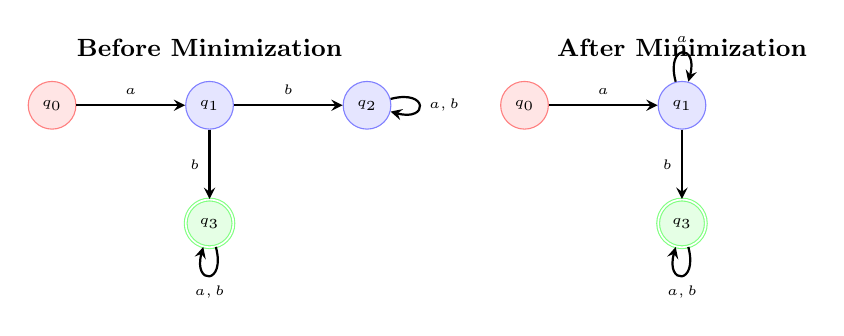
\begin{tikzpicture}[
        state/.style={circle, draw=blue!50, fill=blue!10, minimum size=0.6cm, font=\tiny},
        accept/.style={circle, draw=green!50, fill=green!10, minimum size=0.6cm, font=\tiny, double},
        start/.style={circle, draw=red!50, fill=red!10, minimum size=0.6cm, font=\tiny},
        arrow/.style={->, >=stealth, thick},
        node distance=1.5cm
    ]
    
    % Before minimization
    \node[font=\small, above=0.5cm] at (0,0) {\textbf{Before Minimization}};
    \node[start] (q0a) at (-2,0) {$q_0$};
    \node[state] (q1a) at (0,0) {$q_1$};
    \node[state] (q2a) at (2,0) {$q_2$};
    \node[accept] (q3a) at (0,-1.5) {$q_3$};
    
    \draw[arrow] (q0a) -- node[above, font=\tiny] {$a$} (q1a);
    \draw[arrow] (q1a) -- node[above, font=\tiny] {$b$} (q2a);
    \draw[arrow] (q2a) to[loop right] node[right, font=\tiny] {$a,b$} (q2a);
    \draw[arrow] (q1a) -- node[left, font=\tiny] {$b$} (q3a);
    \draw[arrow] (q3a) to[loop below] node[below, font=\tiny] {$a,b$} (q3a);
    
    % After minimization
    \node[font=\small, above=0.5cm] at (6,0) {\textbf{After Minimization}};
    \node[start] (q0b) at (4,0) {$q_0$};
    \node[state] (q1b) at (6,0) {$q_1$};
    \node[accept] (q3b) at (6,-1.5) {$q_3$};
    
    \draw[arrow] (q0b) -- node[above, font=\tiny] {$a$} (q1b);
    \draw[arrow] (q1b) -- node[left, font=\tiny] {$b$} (q3b);
    \draw[arrow] (q1b) to[loop above] node[above, font=\tiny] {$a$} (q1b);
    \draw[arrow] (q3b) to[loop below] node[below, font=\tiny] {$a,b$} (q3b);
    
    \end{tikzpicture}%
    }
    \caption{Contoh DFA sebelum dan sesudah minimisasi (state $q_2$ dihapus karena equivalent dengan $q_1$)}
    \label{fig:dfa-minimization}
\end{figure}

\subsection{Konsep State Equivalence}

Dua states dalam DFA dikatakan \textbf{equivalent} jika:
\begin{itemize}
    \item Keduanya accept states ATAU keduanya bukan accept states
    \item Untuk setiap input symbol, transisi dari kedua states menuju ke states yang equivalent
\end{itemize}

\subsection{Algoritma Minimization}

Algoritma minimisasi bekerja dengan:
\begin{enumerate}
    \item Partisi states menjadi dua grup: accept states dan non-accept states
    \item Untuk setiap partisi, periksa apakah states dalam partisi tersebut equivalent
    \item Jika tidak equivalent, pisahkan menjadi partisi baru
    \item Ulangi sampai tidak ada partisi yang dapat dipisah lagi
    \item Merge states dalam partisi yang sama
\end{enumerate}

DFA yang sudah diminimalkan memiliki jumlah states minimum yang masih ekuivalen dengan DFA asli.